% =====================================================================
% PyCore Execution Flow Specification
% End-to-end path: Python source → CPython image → hardware retirement
% =====================================================================
\documentclass[11pt,a4paper]{article}

% ---- Packages --------------------------------------------------------
\usepackage[margin=1in]{geometry}
\usepackage{lmodern}
\usepackage[T1]{fontenc}
\usepackage{microtype}
\usepackage{booktabs}
\usepackage{tabularx}
\usepackage{longtable}
\usepackage{array}
\usepackage{enumitem}
\usepackage{xcolor}
\usepackage{graphicx}
\usepackage{hyperref}
\usepackage{amsmath,amssymb}
\usepackage{listings}
\usepackage{fancyvrb}
\usepackage{tikz}
\usepackage{pgfplots}
\pgfplotsset{compat=1.18}
\usetikzlibrary{
  arrows.meta, positioning, shapes.geometric, shapes.multipart,
  fit, calc, chains, decorations.pathreplacing, backgrounds,
  matrix, shadows, patterns, mindmap, trees, automata, shadows.blur
}
\usepackage[most]{tcolorbox}
\usepackage{caption}
\usepackage{subcaption}
\usepackage{fancyhdr}
\usepackage{titlesec}
\usepackage{tocloft}

% ---- Colors ----------------------------------------------------------
\definecolor{pcBlue}{HTML}{1B4F72}
\definecolor{pcTeal}{HTML}{0E6655}
\definecolor{pcAmber}{HTML}{B9770E}
\definecolor{pcRed}{HTML}{922B21}
\definecolor{pcGray}{HTML}{566573}
\definecolor{pcLight}{HTML}{EBF5FB}
\definecolor{pcSoft}{HTML}{F4F6F7}
\definecolor{pcCode}{HTML}{1C2833}
\definecolor{pcImem}{HTML}{1A5276}
\definecolor{pcDmem}{HTML}{196F3D}
\definecolor{pcHost}{HTML}{6C3483}
\definecolor{pcHw}{HTML}{1B4F72}
\definecolor{pcTrap}{HTML}{922B21}

% ---- Hyperref / headers ---------------------------------------------
\hypersetup{
  colorlinks=true,
  linkcolor=pcBlue,
  urlcolor=pcTeal,
  citecolor=pcBlue,
  pdftitle={PyCore Execution Flow Specification},
  pdfauthor={PyCore Project}
}
\pagestyle{fancy}
\fancyhf{}
\fancyhead[L]{\small\textsc{PyCore Execution Flow Specification}}
\fancyhead[R]{\small\thepage}
\fancyfoot[C]{\footnotesize\texttt{pycore/docs/pycore\_execution\_flow.tex}}
\renewcommand{\headrulewidth}{0.4pt}

\titleformat{\section}{\Large\bfseries\color{pcBlue}}{\thesection}{1em}{}
\titleformat{\subsection}{\large\bfseries\color{pcTeal}}{\thesubsection}{1em}{}
\titleformat{\subsubsection}{\normalsize\bfseries\color{pcGray}}{\thesubsubsection}{1em}{}

% ---- Boxes -----------------------------------------------------------
\newtcolorbox{specbox}[1][]{%
  colback=pcLight, colframe=pcBlue, fonttitle=\bfseries,
  title=#1, boxrule=0.6pt, arc=2pt, left=6pt, right=6pt, top=4pt, bottom=4pt
}
\newtcolorbox{normbox}[1][]{%
  colback=pcSoft, colframe=pcGray, fonttitle=\bfseries,
  title=#1, boxrule=0.5pt, arc=2pt, left=6pt, right=6pt, top=4pt, bottom=4pt
}
\newtcolorbox{warnbox}[1][]{%
  colback=yellow!8, colframe=pcAmber, fonttitle=\bfseries,
  title=#1, boxrule=0.6pt, arc=2pt, left=6pt, right=6pt, top=4pt, bottom=4pt
}
\newtcolorbox{trapbox}[1][]{%
  colback=red!5, colframe=pcTrap, fonttitle=\bfseries,
  title=#1, boxrule=0.6pt, arc=2pt, left=6pt, right=6pt, top=4pt, bottom=4pt
}

% ---- Listings --------------------------------------------------------
\lstdefinestyle{pycore}{
  basicstyle=\ttfamily\small\color{pcCode},
  keywordstyle=\bfseries\color{pcBlue},
  commentstyle=\itshape\color{pcGray},
  stringstyle=\color{pcTeal},
  showstringspaces=false,
  breaklines=true,
  frame=single,
  rulecolor=\color{pcGray!40},
  backgroundcolor=\color{pcSoft},
  columns=fullflexible,
  keepspaces=true,
  tabsize=2
}
\lstset{style=pycore}
\lstdefinestyle{python}{
  language=Python,
  style=pycore,
  morekeywords={managed_entry, True, False, None}
}
\lstdefinestyle{hex}{
  style=pycore,
  comment=[l]{\#}
}

% ---- Helpers ---------------------------------------------------------
\newcommand{\opcode}[1]{\texttt{\textbf{#1}}}
\newcommand{\tagname}[1]{\texttt{#1}}
\newcommand{\modname}[1]{\texttt{#1}}
\newcommand{\hexaddr}[1]{\texttt{0x#1}}
\newcommand{\bitfield}[1]{\texttt{#1}}

\begin{document}

% =====================================================================
\begin{titlepage}
\centering
\vspace*{1.5cm}
{\Huge\bfseries\color{pcBlue} PyCore}\\[0.4cm]
{\LARGE Execution Flow Specification}\\[1.2cm]
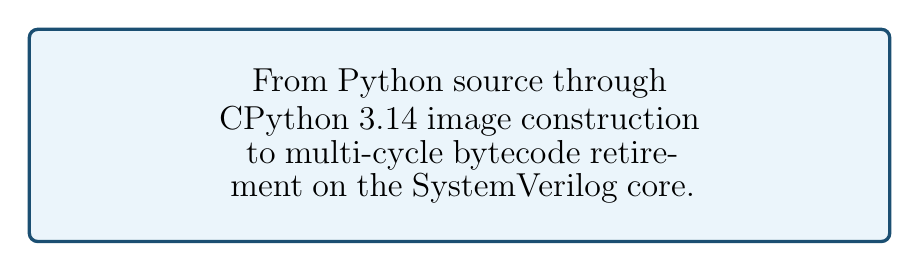
\begin{tikzpicture}
  \node[draw=pcBlue, line width=1.2pt, rounded corners=3pt,
        fill=pcLight, inner sep=14pt, text width=0.82\textwidth, align=center] {
    \large From Python source through CPython~3.14 image construction\\
    to multi-cycle bytecode retirement on the SystemVerilog core.
  };
\end{tikzpicture}\\[1.5cm]
\begin{tabular}{@{}ll@{}}
  \textbf{Document type} & Normative technical specification \\
  \textbf{Scope}         & Host tooling + RTL control/datapath \\
  \textbf{ISA}           & CPython 3.14 bytecode subset \\
  \textbf{Value model}   & Tagged 132-bit entries $\{\mathrm{tag}[3{:}0],\mathrm{value}[127{:}0]\}$ \\
  \textbf{Primary path}  & \texttt{image\_from\_source.py} $\rightarrow$ \texttt{pycore\_system} \\
  \textbf{Companion docs}& \texttt{architecture.md}, \texttt{bytecode\_support.md},
                           \texttt{preprocessing\_breakdown.md} \\
\end{tabular}\\[2cm]
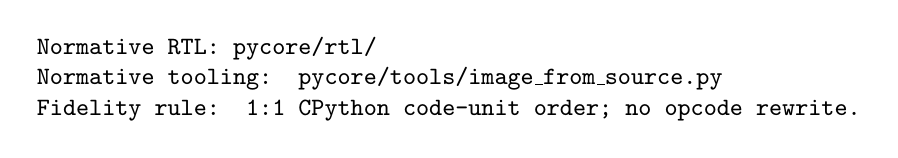
\begin{tikzpicture}
\node[font=\small\ttfamily, align=left] {
  Normative RTL: \texttt{pycore/rtl/}\\
  Normative tooling: \texttt{pycore/tools/image\_from\_source.py}\\
  Fidelity rule: 1:1 CPython code-unit order; no opcode rewrite.
};
\end{tikzpicture}
\vfill
{\large Version aligned to repository \texttt{main} / PyCore image-boot path}\\[0.3cm]
{\normalsize \today}
\end{titlepage}

\tableofcontents
\newpage

% =====================================================================
\section{Purpose and Normative Scope}
\label{sec:scope}

This document specifies the complete execution path of a Python program on
\textbf{PyCore}: a research CPU whose native ISA is a subset of CPython~3.14
bytecode. It is written so that a reader unfamiliar with the repository can
reconstruct, from this specification alone:

\begin{enumerate}[leftmargin=*]
  \item how host-side tooling turns \texttt{.py} source into memory images;
  \item how those images are laid out in instruction and data memory;
  \item how reset bootstraps a module code object and globals dictionary;
  \item how each bytecode walks the multi-cycle control FSM to retirement;
  \item how tags, traps, frames, and containers interact with that FSM.
\end{enumerate}

\begin{specbox}[Normative sources of truth]
\begin{itemize}[leftmargin=*,itemsep=2pt]
  \item \textbf{RTL}: \modname{pycore\_defs.svh}, \modname{pycore\_core.sv},
        \modname{pycore\_fetch.sv}, \modname{pycore\_decode.sv},
        \modname{pycore\_exec.sv}, \modname{pycore\_frame.sv},
        \modname{pycore\_system.sv}.
  \item \textbf{Image builder}: \modname{pycore/tools/image\_from\_source.py}
        (primary). \modname{preprocess.py} is legacy and out of scope for new
        image-boot programs.
  \item \textbf{Encoding helpers}: \modname{encoding.py}, \modname{heap\_image.py}.
\end{itemize}
\end{specbox}

\begin{warnbox}[Fidelity boundary]
``Identical to what a CPython compiler would create'' means: the image contains
the same object graph as \texttt{compile()} output---same bytecode units in the
same order (including \opcode{CACHE} and \opcode{EXTENDED\_ARG}), same
\texttt{co\_consts}/\texttt{co\_names}, and nested code objects---lowered
mechanically into tagged 128-bit-slot encoding. \emph{No opcode is added,
removed, reordered, rewritten, or argument-remapped.} Byte-exact CPython
C-struct layout is out of scope.
\end{warnbox}

% =====================================================================
\section{End-to-End Pipeline Overview}
\label{sec:overview}

Figure~\ref{fig:e2e} is the master flow. Everything else in this document
refines one stage of this pipeline.

\begin{figure}[htbp]
\centering
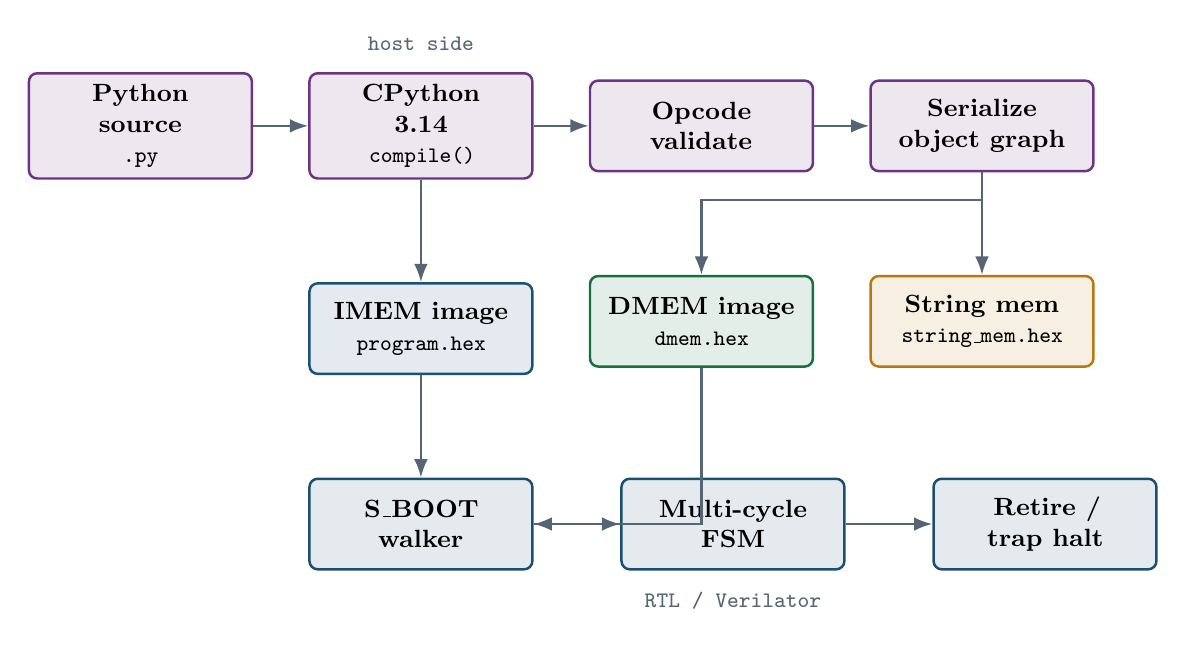
\begin{tikzpicture}[
  node distance=0.55cm and 0.7cm,
  stage/.style={draw=#1, fill=#1!12, line width=0.9pt, rounded corners=3pt,
                align=center, font=\small\bfseries, minimum height=1.15cm,
                text width=2.55cm, inner sep=4pt},
  arr/.style={-{Latex}, thick, color=pcGray},
  note/.style={font=\footnotesize\ttfamily, align=center, text=pcGray}
]
  % Host
  \node[stage=pcHost] (src) {Python\\source\\{\footnotesize\normalfont\texttt{.py}}};
  \node[stage=pcHost, right=of src] (compile) {CPython\\3.14\\{\footnotesize\normalfont\texttt{compile()}}};
  \node[stage=pcHost, right=of compile] (validate) {Opcode\\validate};
  \node[stage=pcHost, right=of validate] (ser) {Serialize\\object graph};
  % Artifacts
  \node[stage=pcImem, below=1.3cm of compile] (imem) {IMEM image\\{\footnotesize\normalfont\texttt{program.hex}}};
  \node[stage=pcDmem, below=1.3cm of validate] (dmem) {DMEM image\\{\footnotesize\normalfont\texttt{dmem.hex}}};
  \node[stage=pcAmber, below=1.3cm of ser] (str) {String mem\\{\footnotesize\normalfont\texttt{string\_mem.hex}}};
  % Hardware
  \node[stage=pcHw, below=1.3cm of imem] (boot) {S\_BOOT\\walker};
  \node[stage=pcHw, right=1.1cm of boot] (fsm) {Multi-cycle\\FSM};
  \node[stage=pcHw, right=1.1cm of fsm] (retire) {Retire /\\trap halt};

  \draw[arr] (src) -- (compile);
  \draw[arr] (compile) -- (validate);
  \draw[arr] (validate) -- (ser);
  \draw[arr] (compile.south) -- (imem.north);
  \draw[arr] (ser.south) -- ++(0,-0.35) -| (dmem.north);
  \draw[arr] (ser.south) -- ++(0,-0.35) -| (str.north);
  \draw[arr] (imem) -- (boot);
  \draw[arr] (dmem.south) |- (boot.east);
  \draw[arr] (boot) -- (fsm);
  \draw[arr] (fsm) -- (retire);

  \node[note, above=0.15cm of compile] {host side};
  \node[note, below=0.15cm of fsm] {RTL / Verilator};
\end{tikzpicture}
\caption{Master pipeline from Python source to instruction retirement.}
\label{fig:e2e}
\end{figure}

\begin{normbox}[Operational contract]
\begin{enumerate}[leftmargin=*,itemsep=1pt]
  \item Host tooling \emph{must} run under Python~3.14 (hard version gate).
  \item Unsupported / deferred opcodes \emph{must} be rejected before image
        emission when possible.
  \item Hardware treats any remaining illegal opcode as
        \texttt{PY\_TRAP\_ILLEGAL\_OPCODE} and enters \texttt{S\_HALT}.
  \item There is no software fallback interpreter on-core.
\end{enumerate}
\end{normbox}

% =====================================================================
\section{Host-Side Image Construction}
\label{sec:host}

\subsection{Tool chain roles}

\begin{center}
\begin{tabular}{@{}llp{7.2cm}@{}}
\toprule
\textbf{Module} & \textbf{Role} & \textbf{Normative behavior} \\
\midrule
\texttt{image\_from\_source.py} & Primary builder &
  \texttt{compile} $\rightarrow$ validate $\rightarrow$ 1:1 imem transcode
  $\rightarrow$ serialize heap $\rightarrow$ boot record \\
\texttt{encoding.py} & Tag codec & Mirrors \texttt{pycore\_defs.svh} tags;
  short/long string packing; imem slot formatting \\
\texttt{heap\_image.py} & DMEM serializer & LIST/DICT/TUPLE/code-object layouts
  identical to RTL helpers \\
\texttt{run\_image\_test.py} & Differential harness & Runs
  \texttt{managed\_entry()} on host; writes expected tag/value into meta \\
\texttt{preprocess.py} & \emph{Legacy} & Branch remap / CACHE strip / inline
  \opcode{LOAD\_CONST}; \textbf{not} for new image-boot tests \\
\bottomrule
\end{tabular}
\end{center}

\subsection{Builder algorithm}

Figure~\ref{fig:builder} details the host algorithm implemented by
\modname{image\_from\_source.py}.

\begin{figure}[htbp]
\centering
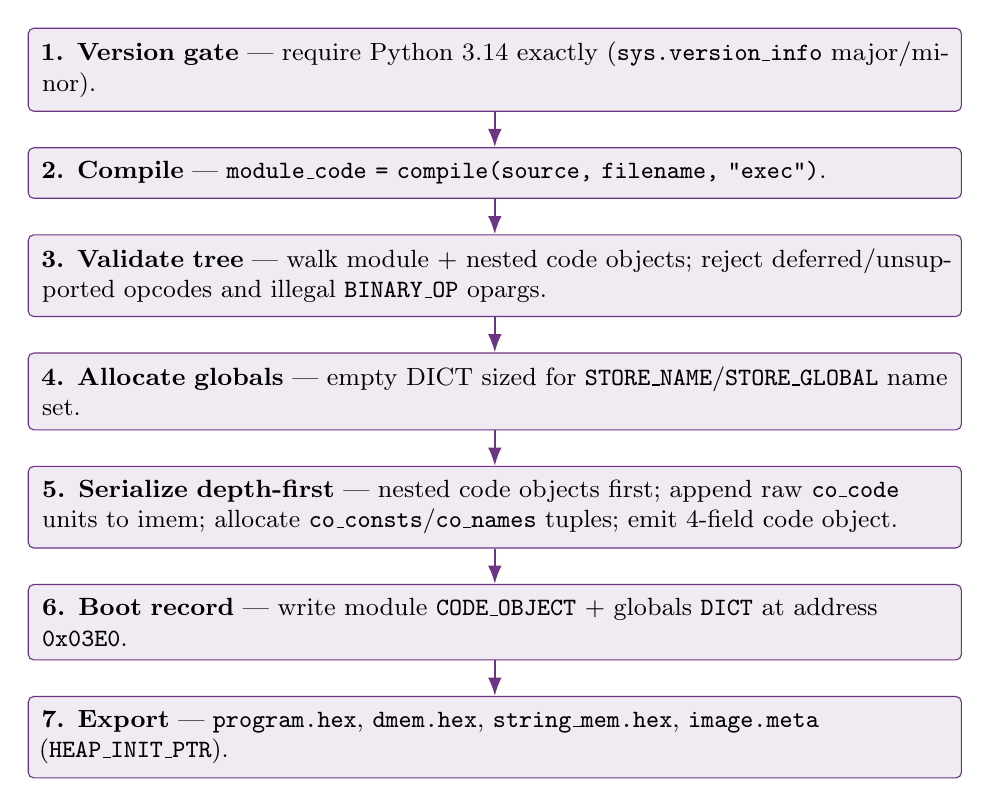
\begin{tikzpicture}[
  node distance=0.45cm,
  flowstep/.style={draw=pcHost, fill=pcHost!10, rounded corners=2pt,
               align=left, font=\small, text width=11.5cm, inner sep=5pt},
  arr/.style={-{Latex}, thick, color=pcHost}
]
  \node[flowstep] (s1) {\textbf{1. Version gate} --- require Python 3.14 exactly (\texttt{sys.version\_info} major/minor).};
  \node[flowstep, below=of s1] (s2) {\textbf{2. Compile} --- \texttt{module\_code = compile(source, filename, "exec")}.};
  \node[flowstep, below=of s2] (s3) {\textbf{3. Validate tree} --- walk module + nested code objects; reject deferred/unsupported opcodes and illegal \texttt{BINARY\_OP} opargs.};
  \node[flowstep, below=of s3] (s4) {\textbf{4. Allocate globals} --- empty DICT sized for \texttt{STORE\_NAME}/\texttt{STORE\_GLOBAL} name set.};
  \node[flowstep, below=of s4] (s5) {\textbf{5. Serialize depth-first} --- nested code objects first; append raw \texttt{co\_code} units to imem; allocate \texttt{co\_consts}/\texttt{co\_names} tuples; emit 4-field code object.};
  \node[flowstep, below=of s5] (s6) {\textbf{6. Boot record} --- write module \texttt{CODE\_OBJECT} + globals \texttt{DICT} at address \texttt{0x03E0}.};
  \node[flowstep, below=of s6] (s7) {\textbf{7. Export} --- \texttt{program.hex}, \texttt{dmem.hex}, \texttt{string\_mem.hex}, \texttt{image.meta} (\texttt{HEAP\_INIT\_PTR}).};

  \draw[arr] (s1) -- (s2);
  \draw[arr] (s2) -- (s3);
  \draw[arr] (s3) -- (s4);
  \draw[arr] (s4) -- (s5);
  \draw[arr] (s5) -- (s6);
  \draw[arr] (s6) -- (s7);
\end{tikzpicture}
\caption{Host image-builder control flow (\texttt{image\_from\_source.py}).}
\label{fig:builder}
\end{figure}

\subsection{Instruction memory slot encoding}

Each CPython two-byte code unit $(opcode, arg8)$ becomes one 64-bit imem slot:

\begin{equation}
  \mathrm{slot} = \{\,0^{24},\; \mathrm{arg}[31{:}0],\; \mathrm{opcode}[7{:}0]\,\}
  \quad\text{stored as 16 hex digits.}
\end{equation}

In practice \texttt{format\_imem\_slot} packs \texttt{bits[39:8]=arg},
\texttt{bits[7:0]=opcode}. Slot index $i$ equals CPython code-unit index $i$;
relative jump arguments are therefore the compiler's original arguments.

\begin{specbox}[CACHE and EXTENDED\_ARG policy]
Both remain \emph{present} in the image. Fetch folds \opcode{EXTENDED\_ARG}
streams and skips \opcode{CACHE} units at execution time. Preprocessing must
not strip them on the image-boot path.
\end{specbox}

\subsection{Object-graph serialization}

Constants are lowered by tag:

\begin{center}
\begin{tabular}{@{}lll@{}}
\toprule
\textbf{Python value} & \textbf{Tag} & \textbf{Value encoding} \\
\midrule
\texttt{int} (fast path) & \tagname{INT} & sign-extended / masked to 128 bits \\
\texttt{float} & \tagname{FLOAT} & IEEE~754 binary64 in \bitfield{value[63:0]} \\
\texttt{bool} & \tagname{BOOL} & \bitfield{value[0]} \\
\texttt{None} & \tagname{NONE} & 0 \\
\texttt{str} $\le 15$ B UTF-8 & \tagname{SHORT\_STR} & size+payload+flags inline \\
\texttt{str} $> 15$ B & \tagname{LONG\_STR} & $\{\mathrm{size},\mathrm{addr}\}$ + string mem \\
\texttt{tuple} & \tagname{TUPLE} & $\{\mathrm{size},\mathrm{addr}\}$ element array \\
\texttt{code} & \tagname{CODE\_OBJECT} & 4-field descriptor (below) \\
\bottomrule
\end{tabular}
\end{center}

Code-object fields (32 bytes each = value slot + tag slot):

\begin{center}
\begin{tabular}{@{}cll@{}}
\toprule
\textbf{Field} & \textbf{Tag} & \textbf{Contents} \\
\midrule
0 & \tagname{INT} & \texttt{entry\_slot} (imem slot index) \\
1 & \tagname{TUPLE} & \texttt{co\_consts} handle \\
2 & \tagname{TUPLE} & \texttt{co\_names} handle \\
3 & \tagname{INT} & packed $\{\mathrm{stacksize},\mathrm{nlocals},\mathrm{argcount}\}$ \\
\bottomrule
\end{tabular}
\end{center}

\subsection{Worked host example}

Consider the minimal program:

\begin{lstlisting}[style=python,caption={pycore/programs/smoke\_return.py}]
def managed_entry() -> int:
    return 12
\end{lstlisting}

\begin{enumerate}[leftmargin=*]
  \item Module bytecode defines \texttt{managed\_entry}, stores it into globals,
        then typically loads and calls it (exact module prologue depends on
        CPython~3.14 wordcode for the module body).
  \item Nested function code object is serialized first: its \texttt{co\_code}
        is appended to imem; \texttt{co\_consts} contains the integer~12.
  \item Module code object follows; globals DICT is empty at image time and
        filled by runtime \opcode{STORE\_NAME}.
  \item Boot record points at the \emph{module} code object and the globals
        DICT.
\end{enumerate}

% =====================================================================
\section{System Topology}
\label{sec:system}

PyCore is a Harvard machine. The simulation top
\modname{pycore\_system} wires the core as a memory master to separate imem
and dmem banks (Figure~\ref{fig:system}).

\begin{figure}[htbp]
\centering
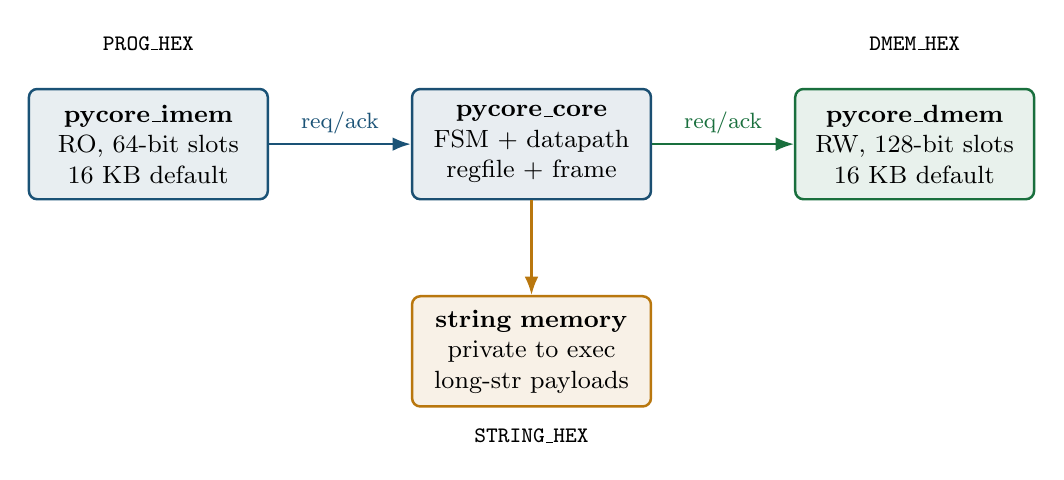
\begin{tikzpicture}[
  box/.style={draw=#1, fill=#1!10, line width=0.9pt, rounded corners=3pt,
              align=center, font=\small, minimum height=1.4cm, text width=2.8cm},
  bus/.style={-{Latex}, thick}
]
  \node[box=pcHw] (core) {\textbf{pycore\_core}\\FSM + datapath\\regfile + frame};
  \node[box=pcImem, left=1.8cm of core] (imem) {\textbf{pycore\_imem}\\RO, 64-bit slots\\16~KB default};
  \node[box=pcDmem, right=1.8cm of core] (dmem) {\textbf{pycore\_dmem}\\RW, 128-bit slots\\16~KB default};
  \node[box=pcAmber, below=1.2cm of core] (str) {\textbf{string memory}\\private to exec\\long-str payloads};

  \draw[bus, pcImem] (imem) -- node[above,font=\footnotesize]{req/ack} (core);
  \draw[bus, pcDmem] (core) -- node[above,font=\footnotesize]{req/ack} (dmem);
  \draw[bus, pcAmber] (core) -- (str);

  \node[font=\footnotesize\ttfamily, above=0.35cm of imem] {PROG\_HEX};
  \node[font=\footnotesize\ttfamily, above=0.35cm of dmem] {DMEM\_HEX};
  \node[font=\footnotesize\ttfamily, below=0.15cm of str] {STRING\_HEX};
\end{tikzpicture}
\caption{Harvard system topology (\texttt{pycore\_system}).}
\label{fig:system}
\end{figure}

\subsection{Memory map (data memory)}

Default parameters: \texttt{ADDR\_WIDTH=32}, \texttt{BLOCK\_SHIFT=12},
4 imem blocks + 4 dmem blocks (16~KB each).

\begin{figure}[htbp]
\centering
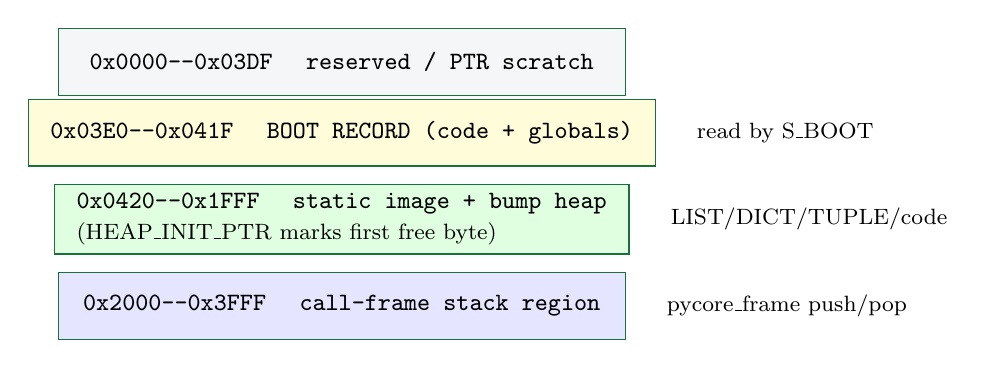
\begin{tikzpicture}[
  cell/.style={draw=pcDmem, fill=#1, minimum width=7.2cm, minimum height=0.85cm,
               align=left, font=\small\ttfamily, inner xsep=8pt},
]
  \node[cell=pcSoft] (r0) at (0,3.6) {0x0000--0x03DF \; reserved / PTR scratch};
  \node[cell=yellow!15] (boot) at (0,2.7) {0x03E0--0x041F \; BOOT RECORD (code + globals)};
  \node[cell=green!12] (heap) at (0,1.6) {0x0420--0x1FFF \; static image + bump heap\\
    \footnotesize\normalfont (HEAP\_INIT\_PTR marks first free byte)};
  \node[cell=blue!10] (frame) at (0,0.5) {0x2000--0x3FFF \; call-frame stack region};

  \node[font=\footnotesize, right=0.4cm of boot] {read by S\_BOOT};
  \node[font=\footnotesize, right=0.4cm of heap] {LIST/DICT/TUPLE/code};
  \node[font=\footnotesize, right=0.4cm of frame] {pycore\_frame push/pop};
\end{tikzpicture}
\caption{DMEM address map (normative defaults from \texttt{pycore\_defs.svh}).}
\label{fig:memmap}
\end{figure}

\begin{normbox}[Boot record layout]
At \texttt{PYCORE\_BOOT\_RECORD\_ADDR = 0x03E0}:
\begin{verbatim}
0x3E0: module code object value
0x3F0: module code object tag
0x400: globals dict value
0x410: globals dict tag
\end{verbatim}
Static heap allocations begin at $\max(\texttt{HEAP\_BASE},\;
\texttt{BOOT\_RECORD\_ADDR}+64)$ so they do not collide with the boot record.
\end{normbox}

% =====================================================================
\section{Tagged Value Model}
\label{sec:tags}

Every architectural value is a 132-bit register-file entry:

\begin{equation}
  E = \{\,\mathrm{tag}[3{:}0],\; \mathrm{value}[127{:}0]\,\}.
\end{equation}

When stored in DMEM, $E$ is split across two consecutive 16-byte slots
(value first, then tag in \bitfield{[3:0]} of the second slot). This keeps all
dmem addressing 16-byte aligned.

\begin{figure}[htbp]
\centering
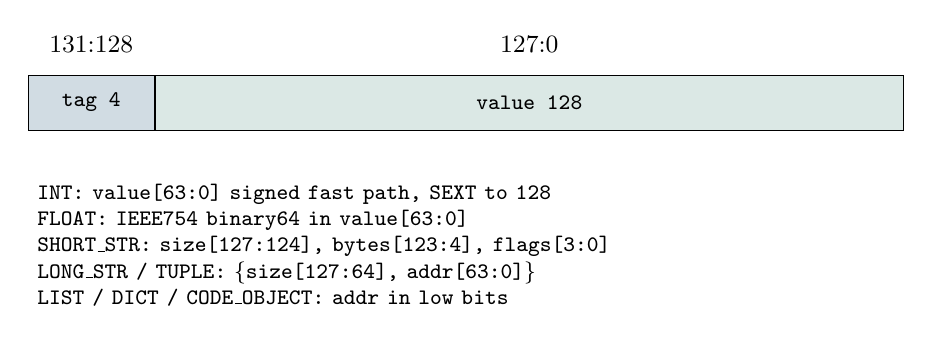
\begin{tikzpicture}[
  bit/.style={draw, minimum height=0.7cm, font=\ttfamily\footnotesize, inner sep=2pt},
]
  \node[bit, fill=pcBlue!20, minimum width=1.6cm] (t) {tag 4};
  \node[bit, fill=pcTeal!15, minimum width=9.5cm, right=0pt of t] (v) {value 128};
  \node[font=\small, above=0.15cm of t] {131:128};
  \node[font=\small, above=0.15cm of v] {127:0};

  \node[font=\footnotesize\ttfamily, align=left, text width=11cm,
        below=0.55cm of t.south west, anchor=north west] {
    INT: value[63:0] signed fast path, SEXT to 128\\
    FLOAT: IEEE754 binary64 in value[63:0]\\
    SHORT\_STR: size[127:124], bytes[123:4], flags[3:0]\\
    LONG\_STR / TUPLE: \{size[127:64], addr[63:0]\}\\
    LIST / DICT / CODE\_OBJECT: addr in low bits
  };
\end{tikzpicture}
\caption{Tagged entry bit layout.}
\label{fig:tagbits}
\end{figure}

\begin{center}
\begin{tabular}{@{}clp{7.8cm}@{}}
\toprule
\textbf{Code} & \textbf{Tag} & \textbf{Meaning} \\
\midrule
\texttt{0000} & UNINITIALIZED & Undefined local; reads trap \\
\texttt{0001} & INT & Signed 64-bit fast path \\
\texttt{0010} & FLOAT & IEEE~754 double \\
\texttt{0011} & BOOL & Truth in \bitfield{value[0]} \\
\texttt{0100} & PTR & 128-bit byte address (v1 uses low 32) \\
\texttt{0101} & TUPLE & $\{\mathrm{size},\mathrm{addr}\}$ \\
\texttt{0110} & SHORT\_STR & Inline $\le 15$ UTF-8 bytes \\
\texttt{0111} & LONG\_STR & External string-memory descriptor \\
\texttt{1000} & OBJECT & Opaque / unsafe; traps on ops \\
\texttt{1001} & DICT & Heap dict handle \\
\texttt{1010} & LIST & Heap list handle \\
\texttt{1011} & SET & Reserved (deferred) \\
\texttt{1100} & CODE\_OBJECT & Callable code descriptor \\
\texttt{1101} & FRAME\_OBJECT & Reserved frame object tag \\
\texttt{1110} & NULL & CPython \texttt{self\_or\_null} sentinel \\
\texttt{1111} & NONE & Python \texttt{None} \\
\bottomrule
\end{tabular}
\end{center}

% =====================================================================
\section{Register File and Operand Stack}
\label{sec:regfile}

\modname{pycore\_regfile} provides 96 architectural entries:

\begin{figure}[htbp]
\centering
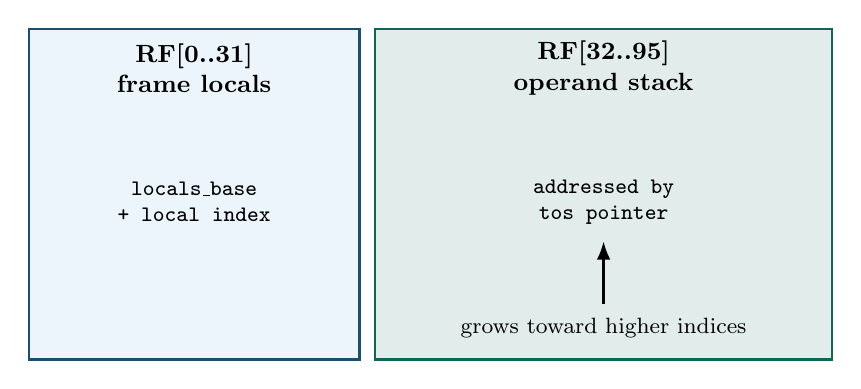
\begin{tikzpicture}
  \fill[pcLight] (0,0) rectangle (4.2,4.2);
  \fill[pcTeal!12] (4.4,0) rectangle (10.2,4.2);
  \draw[thick,pcBlue] (0,0) rectangle (4.2,4.2);
  \draw[thick,pcTeal] (4.4,0) rectangle (10.2,4.2);
  \node[font=\bfseries\small, align=center] at (2.1,3.7) {RF[0..31]\\frame locals};
  \node[font=\bfseries\small, align=center] at (7.3,3.7) {RF[32..95]\\operand stack};
  \node[font=\footnotesize\ttfamily, align=center] at (2.1,2.0) {locals\_base\\+ local index};
  \node[font=\footnotesize\ttfamily, align=center] at (7.3,2.0) {addressed by\\tos pointer};
  \draw[-{Latex}, thick] (7.3,0.7) -- (7.3,1.5);
  \node[font=\footnotesize] at (7.3,0.4) {grows toward higher indices};
\end{tikzpicture}
\caption{Architectural register-file windows.}
\label{fig:rf}
\end{figure}

The operand-stack pointer \texttt{tos} is a core register updated in
\texttt{S\_WB} (or inside \texttt{S\_CONTAINER} for container ops). Decode
reads \texttt{tos} combinationally; because the machine is non-pipelined, no
operand forwarding is required.

% =====================================================================
\section{Control FSM}
\label{sec:fsm}

The core is multi-cycle and non-pipelined: exactly one instruction is in flight.
Figure~\ref{fig:fsm} is the normative state machine from
\modname{pycore\_core.sv}.

\begin{figure}[htbp]
\centering
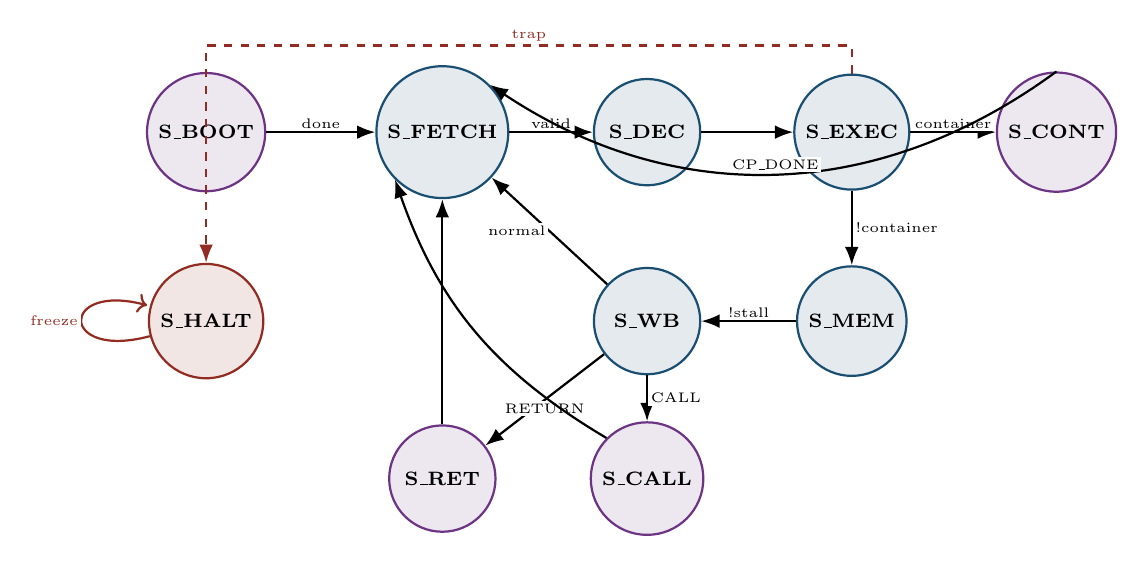
\begin{tikzpicture}[
  state/.style={draw=pcHw, fill=pcHw!12, circle, minimum size=1.35cm,
                font=\scriptsize\bfseries, align=center, line width=0.8pt},
  special/.style={draw=pcHost, fill=pcHost!12, circle, minimum size=1.35cm,
                  font=\scriptsize\bfseries, align=center, line width=0.8pt},
  halt/.style={draw=pcTrap, fill=pcTrap!12, circle, minimum size=1.35cm,
               font=\scriptsize\bfseries, align=center, line width=0.8pt},
  arr/.style={-{Latex}, thick},
  every edge/.style={draw, arr},
  lab/.style={font=\tiny, fill=white, inner sep=1pt}
]
  \node[special] (boot) at (0,0) {S\_BOOT};
  \node[state] (fetch) at (3.0,0) {S\_FETCH};
  \node[state] (decode) at (5.6,0) {S\_DEC};
  \node[state] (exec) at (8.2,0) {S\_EXEC};
  \node[state] (mem) at (8.2,-2.4) {S\_MEM};
  \node[state] (wb) at (5.6,-2.4) {S\_WB};
  \node[special] (cont) at (10.8,0) {S\_CONT};
  \node[special] (call) at (5.6,-4.4) {S\_CALL};
  \node[special] (ret) at (3.0,-4.4) {S\_RET};
  \node[halt] (halt) at (0,-2.4) {S\_HALT};

  \draw[arr] (boot) -- node[lab,above]{done} (fetch);
  \draw[arr] (fetch) -- node[lab,above]{valid} (decode);
  \draw[arr] (decode) -- (exec);
  \draw[arr] (exec) -- node[lab,right]{!container} (mem);
  \draw[arr] (exec) -- node[lab,above]{container} (cont);
  \draw[arr] (mem) -- node[lab,above]{!stall} (wb);
  \draw[arr] (wb) -- node[lab,left]{normal} (fetch);
  \draw[arr] (wb) -- node[lab,right]{CALL} (call);
  \draw[arr] (wb) -- node[lab,below]{RETURN} (ret);
  \draw[arr] (call.north west) to[bend left=20] (fetch.south west);
  \draw[arr] (ret) -- (fetch);
  \draw[arr] (cont.north) to[bend left=35] node[lab,above]{CP\_DONE} (fetch.north east);
  \path[arr,pcTrap] (halt) edge[loop left] node[lab]{freeze} (halt);
  \draw[arr,pcTrap,dashed] (exec) -- ++(0,1.1) -| node[lab,near start,above]{trap} (halt);
\end{tikzpicture}
\caption{PyCore control FSM (states numbered 0--9 in RTL).}
\label{fig:fsm}
\end{figure}

\subsection{State responsibilities}

\begin{description}[style=nextline,leftmargin=1.4cm,font=\ttfamily\bfseries]
  \item[S\_BOOT] When \texttt{BOOT\_EN=1}, read boot record; cache
    \texttt{co\_consts}/\texttt{co\_names}; latch \texttt{globals\_base};
    redirect fetch to module entry slot.
  \item[S\_FETCH] Run \modname{pycore\_fetch} until a real instruction is
    presented; latch $\{\mathrm{opcode},\mathrm{arg},\mathrm{pc}\}$. Fold
    \opcode{EXTENDED\_ARG}; skip \opcode{CACHE}.
  \item[S\_DECODE] Drive RF read addresses; latch operands.
  \item[S\_EXEC] Execute fabric / branch unit; may stall on multi-cycle units.
    If \texttt{dec\_is\_container}, divert to \texttt{S\_CONTAINER}.
  \item[S\_MEM] PTR load/store via \modname{pycore\_mem\_stage}; hold on
    outstanding dmem access.
  \item[S\_WB] Write RF; advance \texttt{tos}; redirect fetch on taken branch;
    enter \texttt{S\_CALL}/\texttt{S\_RETURN} when indicated.
  \item[S\_CONTAINER] Multi-cycle container / name / const path; bypasses
    \texttt{S\_MEM}/\texttt{S\_WB}.
  \item[S\_CALL] / \textbf{S\_RETURN} Frame push/pop + code-object field reload.
  \item[S\_HALT] Terminal freeze on any trap.
\end{description}

\begin{specbox}[Hazard rule]
Because only one instruction is ever in flight, there are \textbf{no pipeline
hazards}. Multi-cycle execute or memory simply holds the FSM in
\texttt{S\_EXEC}/\texttt{S\_MEM} until completion.
\end{specbox}

% =====================================================================
\section{Fetch Stage}
\label{sec:fetch}

\modname{pycore\_fetch} is a registered req/ack imem master. Address formation:

\begin{equation}
  \mathrm{imem\_addr} = \mathrm{pc} \ll 3
  \quad\text{(8-byte slots).}
\end{equation}

\begin{figure}[htbp]
\centering
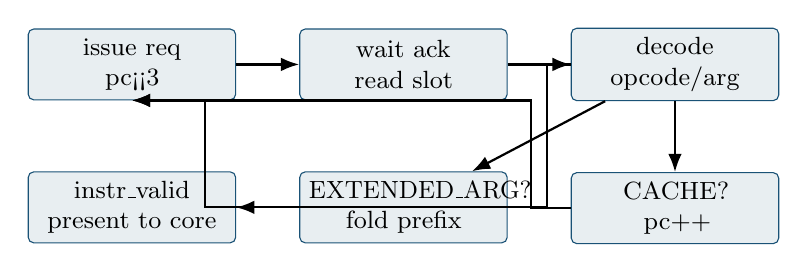
\begin{tikzpicture}[
  box/.style={draw=pcImem, fill=pcImem!10, rounded corners=2pt, align=center,
              font=\small, minimum height=0.9cm, text width=2.4cm},
  arr/.style={-{Latex}, thick}
]
  \node[box] (req) {issue req\\pc<<3};
  \node[box, right=0.8cm of req] (ack) {wait ack\\read slot};
  \node[box, right=0.8cm of ack] (dec) {decode\\opcode/arg};
  \node[box, below=0.9cm of dec] (cache) {CACHE?\\pc++};
  \node[box, below=0.9cm of ack] (ext) {EXTENDED\_ARG?\\fold prefix};
  \node[box, below=0.9cm of req] (valid) {instr\_valid\\present to core};

  \draw[arr] (req) -- (ack);
  \draw[arr] (ack) -- (dec);
  \draw[arr] (dec) -- (cache);
  \draw[arr] (dec) -- (ext);
  \draw[arr] (dec.west) -- ++(-0.3,0) |- (valid);
  \draw[arr] (cache.west) -- ++(-0.5,0) |- (req.south);
  \draw[arr] (ext.west) -- ++(-1.2,0) |- (req.south);
\end{tikzpicture}
\caption{Fetch internal behavior: fold, skip, or present.}
\label{fig:fetch}
\end{figure}

Argument folding:
\begin{equation}
  \mathrm{arg}_{\mathrm{eff}} =
  \begin{cases}
    (\mathrm{prefix}\ll 8)\;|\;\mathrm{arg}[7{:}0] & \text{if prior EXTENDED\_ARG} \\
    \mathrm{arg} & \text{otherwise.}
  \end{cases}
\end{equation}

The core freezes fetch via \texttt{stall} while an instruction is in later
states, and ignores stale \texttt{instr\_valid} until a fresh fetch completes
after re-entering \texttt{S\_FETCH}.

% =====================================================================
\section{Decode Stage}
\label{sec:decode}

\modname{pycore\_decode} is combinational. It maps
$(\mathrm{opcode},\mathrm{arg},\mathrm{tos},\mathrm{locals\_base})$ to:

\begin{itemize}[leftmargin=*]
  \item ALU op / branch / call / return / container class bits;
  \item RF selectors \texttt{rs1}/\texttt{rs2}/\texttt{rd};
  \item stack push/pop effects;
  \item memory op class (\texttt{LOAD\_FAST}/\texttt{STORE\_FAST}/PTR).
\end{itemize}

\begin{figure}[htbp]
\centering
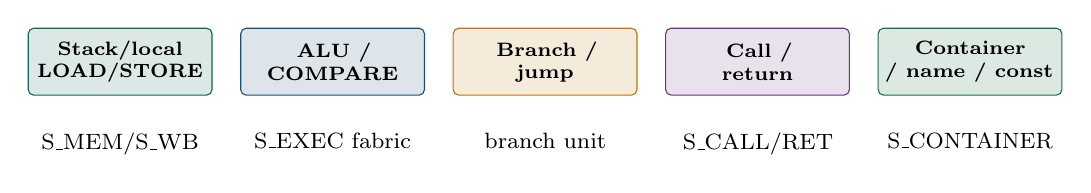
\begin{tikzpicture}[
  op/.style={draw, rounded corners=2pt, fill=#1!15, draw=#1, font=\scriptsize\bfseries,
             align=center, text width=2.1cm, minimum height=0.85cm},
]
  \node[op=pcTeal] (a) {Stack/local\\LOAD/STORE};
  \node[op=pcBlue, right=0.35cm of a] (b) {ALU /\\COMPARE};
  \node[op=pcAmber, right=0.35cm of b] (c) {Branch /\\jump};
  \node[op=pcHost, right=0.35cm of c] (d) {Call /\\return};
  \node[op=pcDmem, right=0.35cm of d] (e) {Container\\/ name / const};

  \node[font=\footnotesize, below=0.35cm of a, text width=2.1cm, align=center] {S\_MEM/S\_WB};
  \node[font=\footnotesize, below=0.35cm of b, text width=2.1cm, align=center] {S\_EXEC fabric};
  \node[font=\footnotesize, below=0.35cm of c, text width=2.1cm, align=center] {branch unit};
  \node[font=\footnotesize, below=0.35cm of d, text width=2.1cm, align=center] {S\_CALL/RET};
  \node[font=\footnotesize, below=0.35cm of e, text width=2.1cm, align=center] {S\_CONTAINER};
\end{tikzpicture}
\caption{Decode classification $\rightarrow$ FSM diversion.}
\label{fig:decode-class}
\end{figure}

Notable CPython~3.14 decode rules baked into RTL:

\begin{itemize}[leftmargin=*]
  \item \opcode{COMPARE\_OP}: selector is $\mathrm{oparg}\gg 5$ (range 0..5).
  \item \opcode{LOAD\_GLOBAL}: $\mathrm{namei}=\mathrm{oparg}\gg 1$; if
        $\mathrm{oparg}\&1$, also push \tagname{NULL}.
  \item \opcode{BINARY\_OP} with oparg \texttt{NB\_SUBSCR=26} sets
        \texttt{PY\_ALU\_SUBSCR} and routes to \texttt{S\_CONTAINER}.
  \item Relative jumps: $\mathrm{target}=\mathrm{pc}+1+n_{\mathrm{cache}}\pm\mathrm{arg}$
        with inline-cache counts from CPython~3.14.
\end{itemize}

% =====================================================================
\section{Execute Fabric}
\label{sec:exec}

The execute stage is a tag-routed fabric (Figure~\ref{fig:exec}).

\begin{figure}[htbp]
\centering
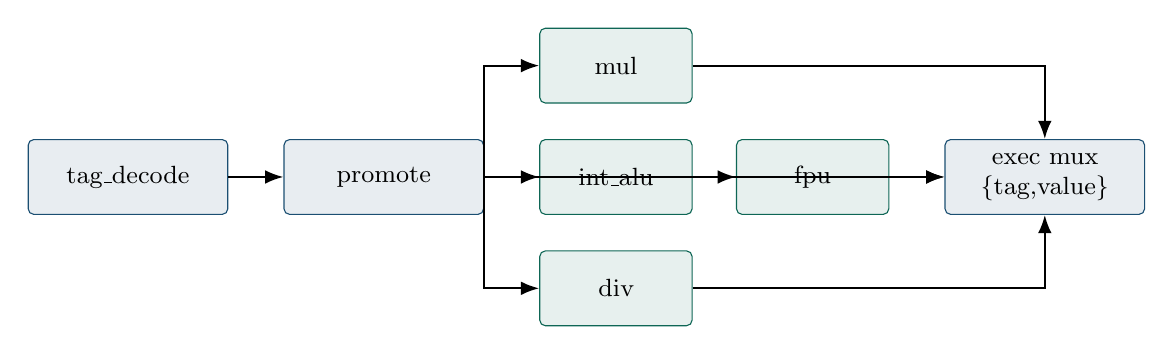
\begin{tikzpicture}[
  box/.style={draw=pcHw, fill=pcHw!10, rounded corners=2pt, align=center,
              font=\small, minimum height=0.95cm, text width=2.3cm},
  unit/.style={draw=pcTeal, fill=pcTeal!10, rounded corners=2pt, align=center,
               font=\small, minimum height=0.95cm, text width=1.7cm},
  arr/.style={-{Latex}, thick}
]
  \node[box] (td) {tag\_decode};
  \node[box, right=0.7cm of td] (pr) {promote};
  \node[unit, right=0.7cm of pr] (alu) {int\_alu};
  \node[unit, above=0.45cm of alu] (mul) {mul};
  \node[unit, below=0.45cm of alu] (div) {div};
  \node[unit, right=0.55cm of alu] (fpu) {fpu};
  \node[box, right=0.7cm of fpu] (mux) {exec mux\\\{tag,value\}};

  \draw[arr] (td) -- (pr);
  \draw[arr] (pr.east) -- (alu.west);
  \draw[arr] (pr.east) |- (mul.west);
  \draw[arr] (pr.east) |- (div.west);
  \draw[arr] (pr.east) |- (fpu.west);
  \draw[arr] (alu) -- (mux);
  \draw[arr] (mul) -| (mux);
  \draw[arr] (div) -| (mux);
  \draw[arr] (fpu) -- (mux);
\end{tikzpicture}
\caption{Tag-routed execute fabric.}
\label{fig:exec}
\end{figure}

Promotion rules selected by tag decode:

\begin{center}
\begin{tabular}{@{}ll@{}}
\toprule
\textbf{Promotion} & \textbf{When} \\
\midrule
\texttt{BOOL $\rightarrow$ INT} & integer ALU path needs numeric \\
\texttt{BOOL $\rightarrow$ FLOAT} / \texttt{INT $\rightarrow$ FLOAT} & true divide or float op \\
\texttt{NB\_TRUE\_DIVIDE} & always yields \tagname{FLOAT} \\
\bottomrule
\end{tabular}
\end{center}

\begin{warnbox}[Semantic deviation --- integers]
Integer add/sub/mul/shift wrap at 64 bits. This is the largest intentional
deviation from CPython arbitrary-precision integers. Programs outside signed
64-bit range can silently diverge unless rejected earlier.
\end{warnbox}

String \opcode{BINARY\_OP (+)} concatenates \tagname{SHORT\_STR}/\tagname{LONG\_STR}
pairs inside the exec unit's private string memory; oversized results raise
\texttt{MEM\_FAULT}.

% =====================================================================
\section{Container Operations}
\label{sec:containers}

\texttt{S\_CONTAINER} handles multi-cycle heap and name operations, entered
directly from \texttt{S\_EXEC} when \texttt{dec\_is\_container} is set. It
bypasses \texttt{S\_MEM} and \texttt{S\_WB}; TOS/RF updates occur inside the
container FSM.

\subsection{Shared phase machine}

\begin{center}
\begin{tabular}{@{}clp{8.5cm}@{}}
\toprule
\textbf{Phase} & \textbf{Name} & \textbf{Purpose} \\
\midrule
0 & \texttt{CP\_INIT} & First active cycle; launch first dmem/RF op \\
1 & \texttt{CP\_HDR}  & Header R/W in flight \\
2 & \texttt{CP\_VAL}  & Element value R/W in flight \\
3 & \texttt{CP\_TAG}  & Element tag R/W in flight \\
4 & \texttt{CP\_DONE} & Terminal; combinational return to \texttt{S\_FETCH} \\
\bottomrule
\end{tabular}
\end{center}

Dict-specific phases extend through \texttt{CP\_DICT\_HASH}..\texttt{CP\_DICT\_RD\_VTAG}
for probe/hash sequences.

\subsection{Heap bump allocator}

\begin{equation}
  \texttt{HEAP\_BASE}=0\times0400,\quad
  \texttt{HEAP\_LIMIT}=0\times2000,\quad
  \text{capacity}\approx 7\,\mathrm{KB}.
\end{equation}

\texttt{heap\_ptr\_r} advances monotonically from \texttt{HEAP\_INIT\_PTR}
(from image meta). Overflow $\Rightarrow$ \texttt{PY\_TRAP\_MEM\_FAULT}.
No free list / GC in this prototype.

\subsection{In-memory layouts}

\begin{figure}[htbp]
\centering
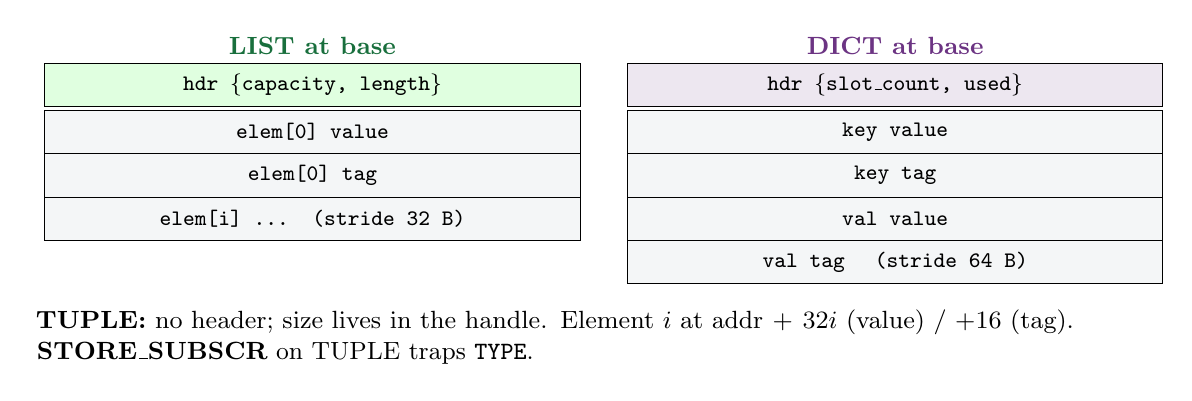
\begin{tikzpicture}[
  slot/.style={draw, minimum width=6.8cm, minimum height=0.55cm,
               font=\ttfamily\footnotesize, align=left, inner xsep=6pt},
]
  % LIST
  \node[font=\bfseries\small\color{pcDmem}] at (0,4.4) {LIST at base};
  \node[slot, fill=green!12] at (0,3.9) {hdr \{capacity, length\}};
  \node[slot, fill=pcSoft] at (0,3.3) {elem[0] value};
  \node[slot, fill=pcSoft] at (0,2.75) {elem[0] tag};
  \node[slot, fill=pcSoft] at (0,2.2) {elem[i] ... (stride 32 B)};

  % DICT
  \begin{scope}[xshift=7.4cm]
  \node[font=\bfseries\small\color{pcHost}] at (0,4.4) {DICT at base};
  \node[slot, fill=pcHost!12] at (0,3.9) {hdr \{slot\_count, used\}};
  \node[slot, fill=pcSoft] at (0,3.3) {key value};
  \node[slot, fill=pcSoft] at (0,2.75) {key tag};
  \node[slot, fill=pcSoft] at (0,2.2) {val value};
  \node[slot, fill=pcSoft] at (0,1.65) {val tag \; (stride 64 B)};
  \end{scope}

  % TUPLE note
  \node[font=\small, text width=14cm, align=left] at (3.5,0.7) {
    \textbf{TUPLE:} no header; size lives in the handle. Element $i$ at
    $\mathrm{addr}+32i$ (value) / $+16$ (tag). \textbf{STORE\_SUBSCR} on TUPLE
    traps \texttt{TYPE}.
  };
\end{tikzpicture}
\caption{Container DMEM layouts (16-byte slot granularity).}
\label{fig:layouts}
\end{figure}

Dict hashing (open-addressed linear probe, tombstone-free):

\begin{center}
\begin{tabular}{@{}ll@{}}
\toprule
\textbf{Key tag} & \textbf{Hash} \\
\midrule
INT / BOOL & \bitfield{value[31:0]} \\
SHORT\_STR & XOR of four 32-bit words of value \\
LONG\_STR & $\mathrm{value}[31{:}0]\oplus\mathrm{value}[95{:}64]$ \\
\bottomrule
\end{tabular}
\end{center}

Slot count at construction: $\mathrm{next\_pow2}(\max(4,\,2\cdot n_{\mathrm{pairs}}))$
(load $\le 50\%$). Empty-bucket sentinel: key tag \tagname{UNINIT}. Inserts that
would fill the table completely trap so probes always terminate.

\subsection{Operations routed to S\_CONTAINER}

\begin{center}
\begin{tabular}{@{}llp{6.8cm}@{}}
\toprule
\textbf{Bytecode} & \textbf{Container op} & \textbf{Behavior} \\
\midrule
\opcode{BUILD\_LIST} & CONT\_BUILD\_LIST & bump-alloc header+elements; push LIST \\
\opcode{BUILD\_TUPLE} & CONT\_BUILD\_TUPLE & alloc elements only; push TUPLE \\
\opcode{BUILD\_MAP} & CONT\_BUILD\_MAP & alloc+probe-insert pairs; push DICT \\
\opcode{BINARY\_OP} NB\_SUBSCR & CONT\_SUBSCR\_* & list/tuple index or dict probe \\
\opcode{STORE\_SUBSCR} & CONT\_STORE\_* & list write or dict upsert \\
\opcode{LOAD\_CONST} & CONT\_LOAD\_CONST & two dmem reads from \texttt{co\_consts} \\
\opcode{LOAD\_GLOBAL}/\opcode{LOAD\_NAME} & name lookup & \texttt{co\_names} then globals probe \\
\opcode{STORE\_NAME}/\opcode{STORE\_GLOBAL} & globals store & upsert into module DICT \\
\bottomrule
\end{tabular}
\end{center}

% =====================================================================
\section{Calls, Frames, and Returns}
\label{sec:calls}

\subsection{Interim function model}

\begin{specbox}[function $\equiv$ CODE\_OBJECT]
\opcode{MAKE\_FUNCTION} checks TOS is \tagname{CODE\_OBJECT} and leaves it in
place. Defaults, annotations, closures, and bound methods are rejected by
tooling / unsupported in hardware.
\end{specbox}

\subsection{CPython 3.14 CALL stack layout}

Bottom $\rightarrow$ top before \opcode{CALL}:
\begin{equation}
  [\mathrm{callable},\; \mathrm{NULL},\; \mathrm{arg}_1,\ldots,\mathrm{arg}_N]
\end{equation}
Non-method calls require sentinel tag \tagname{NULL}. Hardware validates
callable tag and \texttt{argcount}, then enters the frame manager.

\begin{figure}[htbp]
\centering
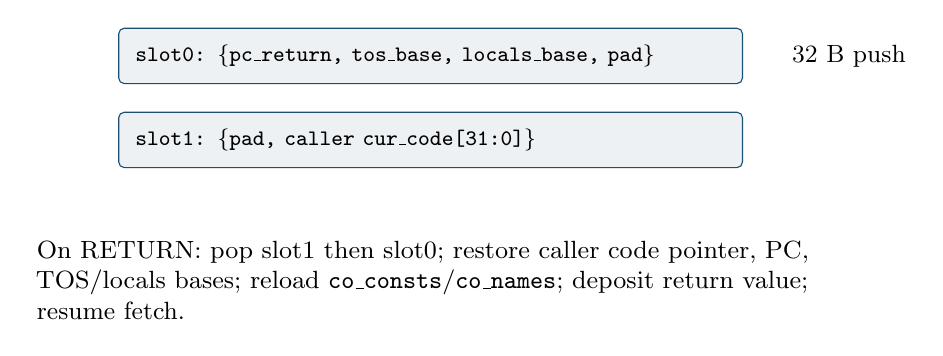
\begin{tikzpicture}[
  frame/.style={draw=pcBlue, fill=pcBlue!8, rounded corners=2pt,
                font=\ttfamily\footnotesize, align=left, text width=7.5cm,
                inner sep=6pt},
  arr/.style={-{Latex}, thick}
]
  \node[frame] (s0) {slot0: \{pc\_return, tos\_base, locals\_base, pad\}};
  \node[frame, below=0.35cm of s0] (s1) {slot1: \{pad, caller cur\_code[31:0]\}};
  \node[font=\small, right=0.5cm of s0] {32 B push};
  \node[font=\small, below=0.8cm of s1, text width=10cm, align=left] {
    On RETURN: pop slot1 then slot0; restore caller code pointer, PC, TOS/locals
    bases; reload \texttt{co\_consts}/\texttt{co\_names}; deposit return value;
    resume fetch.
  };
\end{tikzpicture}
\caption{Call-frame descriptor pushed by \texttt{pycore\_frame}.}
\label{fig:frame}
\end{figure}

Frame depth is bounded by the reserved region \hexaddr{2000}--\hexaddr{3FFF}.
A ring-buffer spill design exists only in \texttt{rtl/attic/} and is
\emph{not} on the production path.

% =====================================================================
\section{Boot Sequence}
\label{sec:boot}

\begin{figure}[htbp]
\centering
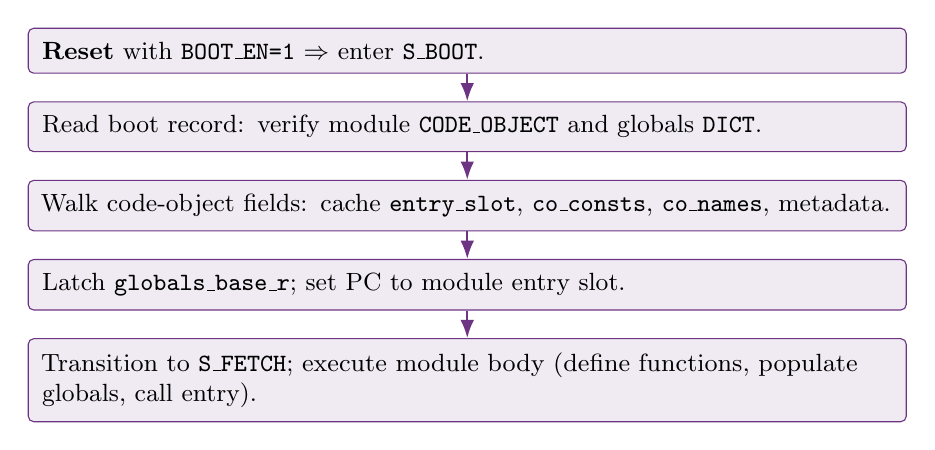
\begin{tikzpicture}[
  flowstep/.style={draw=pcHost, fill=pcHost!10, rounded corners=2pt, align=left,
               font=\small, text width=10.8cm, inner sep=5pt},
  arr/.style={-{Latex}, thick, color=pcHost}
]
  \node[flowstep] (b0) {\textbf{Reset} with \texttt{BOOT\_EN=1} $\Rightarrow$ enter \texttt{S\_BOOT}.};
  \node[flowstep, below=0.35cm of b0] (b1) {Read boot record: verify module \texttt{CODE\_OBJECT} and globals \texttt{DICT}.};
  \node[flowstep, below=0.35cm of b1] (b2) {Walk code-object fields: cache \texttt{entry\_slot}, \texttt{co\_consts}, \texttt{co\_names}, metadata.};
  \node[flowstep, below=0.35cm of b2] (b3) {Latch \texttt{globals\_base\_r}; set PC to module entry slot.};
  \node[flowstep, below=0.35cm of b3] (b4) {Transition to \texttt{S\_FETCH}; execute module body (define functions, populate globals, call entry).};

  \draw[arr] (b0)--(b1);
  \draw[arr] (b1)--(b2);
  \draw[arr] (b2)--(b3);
  \draw[arr] (b3)--(b4);
\end{tikzpicture}
\caption{Image-boot walker.}
\label{fig:boot}
\end{figure}

\texttt{BOOT\_EN=0} remains only for legacy hand-authored hex fixtures that
fetch from PC~0 without a boot record.

% =====================================================================
\section{Trap Architecture}
\label{sec:traps}

\modname{pycore\_trap} latches a trap and forces \texttt{S\_HALT}, freezing
architectural state and the cycle counter. Priority (highest first):

\begin{center}
\begin{tabular}{@{}clp{7.5cm}@{}}
\toprule
\textbf{Pri.} & \textbf{Code} & \textbf{Cause} \\
\midrule
1 & TYPE (1) & Illegal tag for arithmetic/compare/branch/unary; bad dict key tag; store into tuple \\
2 & STACK (2) & Operand-stack overflow/underflow at WB \\
3 & DIV\_ZERO (3) & Integer division by zero \\
4 & FPU\_EXCEPTION (4) & Floating-point exception leaf \\
5 & ILLEGAL\_OPCODE (5) & Decode miss / unsupported opcode \\
6 & CALL\_FILTER (6) & Non-callable, bad argc, frame-manager fault \\
7 & ADDR\_ALIGN (8) & Misaligned dmem access (raised in S\_MEM) \\
8 & MEM\_FAULT (7) & OOR address, missing global/key, bad PTR, heap OOM \\
\bottomrule
\end{tabular}
\end{center}

\begin{trapbox}[No exception objects]
Missing dict keys and undefined globals raise \texttt{MEM\_FAULT}, not Python
\texttt{KeyError}/\texttt{NameError} objects. There is no on-core exception
object protocol in this prototype.
\end{trapbox}

% =====================================================================
\section{Instruction Lifecycle Timeline}
\label{sec:timeline}

Figure~\ref{fig:timeline} shows a generic non-container ALU instruction.

\begin{figure}[htbp]
\centering
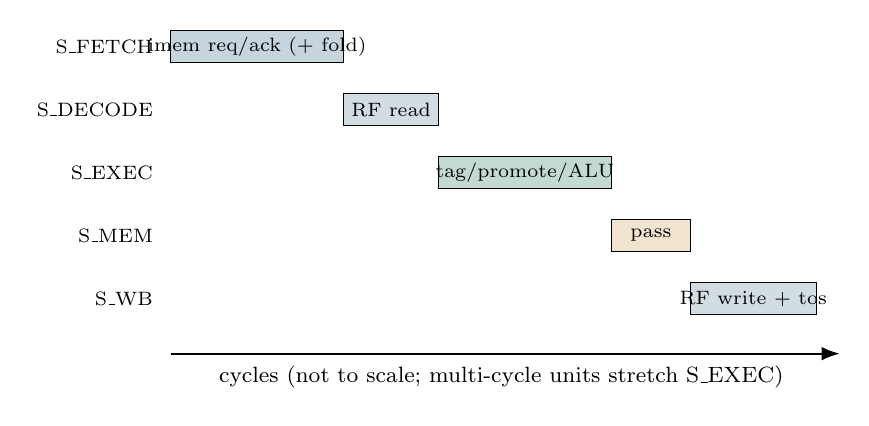
\begin{tikzpicture}[
  every node/.style={font=\scriptsize},
  bar/.style={draw, minimum height=0.55cm, anchor=west, inner sep=2pt, font=\ttfamily\tiny}
]
  \foreach \yy/\lbl in {5.2/S\_FETCH, 4.4/S\_DECODE, 3.6/S\_EXEC, 2.8/S\_MEM, 2.0/S\_WB} {
    \node[anchor=east] at (-0.1,\yy) {\lbl};
  }
  \draw[fill=pcImem!25] (0,5.0) rectangle (2.2,5.4);
  \node at (1.1,5.2) {imem req/ack (+ fold)};
  \draw[fill=pcHw!20] (2.2,4.2) rectangle (3.4,4.6);
  \node at (2.8,4.4) {RF read};
  \draw[fill=pcTeal!25] (3.4,3.4) rectangle (5.6,3.8);
  \node at (4.5,3.6) {tag/promote/ALU};
  \draw[fill=pcAmber!20] (5.6,2.6) rectangle (6.6,3.0);
  \node at (6.1,2.8) {pass};
  \draw[fill=pcBlue!20] (6.6,1.8) rectangle (8.2,2.2);
  \node at (7.4,2.0) {RF write + tos};

  \draw[-{Latex}, thick] (0,1.3) -- (8.5,1.3);
  \node[font=\footnotesize] at (4.2,1.0) {cycles (not to scale; multi-cycle units stretch S\_EXEC)};
\end{tikzpicture}
\caption{Nominal lifecycle of a simple ALU bytecode.}
\label{fig:timeline}
\end{figure}

Container ops replace the MEM/WB tail with an internal phase loop:

\begin{equation}
  \texttt{S\_FETCH}\rightarrow
  \texttt{S\_DECODE}\rightarrow
  \texttt{S\_EXEC}\rightarrow
  \texttt{S\_CONTAINER}(\texttt{CP\_*})\rightarrow
  \texttt{S\_FETCH}.
\end{equation}

% =====================================================================
\section{End-to-End Worked Trace}
\label{sec:trace}

This section walks a concrete path for a module that defines and calls a
function returning a small integer (pattern of \texttt{smoke\_return.py} and
\texttt{img\_smoke.py}).

\begin{figure}[htbp]
\centering
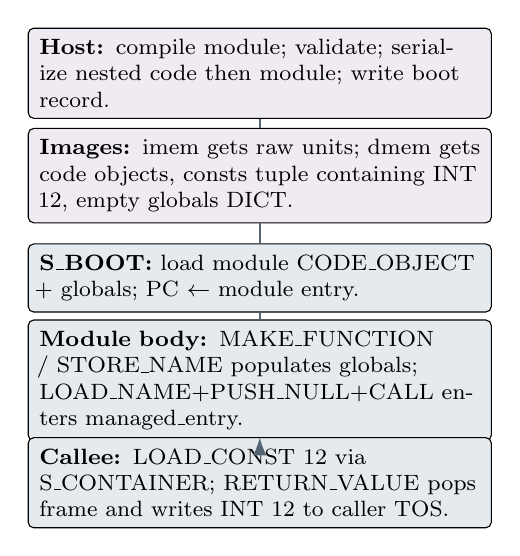
\begin{tikzpicture}[
  n/.style={draw, rounded corners=2pt, align=left, font=\footnotesize,
            text width=5.6cm, inner sep=4pt, fill=#1},
  arr/.style={-{Latex}, thick, pcGray}
]
  \node[n=pcHost!10] (h1) at (0,6.2) {\textbf{Host:} compile module; validate; serialize nested code then module; write boot record.};
  \node[n=pcHost!10] (h2) at (0,4.9) {\textbf{Images:} imem gets raw units; dmem gets code objects, consts tuple containing INT 12, empty globals DICT.};
  \node[n=pcHw!12] (w1) at (0,3.6) {\textbf{S\_BOOT:} load module CODE\_OBJECT + globals; PC $\leftarrow$ module entry.};
  \node[n=pcHw!12] (w2) at (0,2.3) {\textbf{Module body:} MAKE\_FUNCTION / STORE\_NAME populates globals; LOAD\_NAME+PUSH\_NULL+CALL enters managed\_entry.};
  \node[n=pcHw!12] (w3) at (0,1.0) {\textbf{Callee:} LOAD\_CONST 12 via S\_CONTAINER; RETURN\_VALUE pops frame and writes INT 12 to caller TOS.};

  \draw[arr] (h1)--(h2)--(w1)--(w2)--(w3);
\end{tikzpicture}
\caption{Narrative trace from source to returned INT.}
\label{fig:trace}
\end{figure}

\subsection{Per-opcode micro-flows (selected)}

\paragraph{\opcode{LOAD\_CONST}.}
Decode sets \texttt{is\_container}. \texttt{S\_CONTAINER} indexes
\texttt{co\_consts[arg]}, performs value then tag dmem reads, pushes the tagged
entry, returns to fetch.

\paragraph{\opcode{LOAD\_GLOBAL} / \opcode{LOAD\_NAME}.}
Read name string from \texttt{co\_names}; probe module globals DICT; push value;
optionally push \tagname{NULL} when \texttt{oparg\&1}. Missing name $\Rightarrow$
\texttt{MEM\_FAULT}. No builtins fallback.

\paragraph{\opcode{CALL}.}
Validate callable+\tagname{NULL}+argc; read callee code-object fields; push
frame; transfer locals/args; redirect fetch to callee \texttt{entry\_slot}.

\paragraph{\opcode{RETURN\_VALUE}.}
Pop frame; restore caller context; write return entry to caller stack; fetch
resumes at return PC. Base-frame return completes the program (testbench
observes retired value).

\paragraph{\opcode{BINARY\_OP} (arithmetic).}
Pop two stack entries; tag-decode + promote; run int/float unit; push result
tag/value; wrap on 64-bit int overflow.

\paragraph{\opcode{BUILD\_LIST} / \opcode{NB\_SUBSCR}.}
Bump-allocate or index through \texttt{S\_CONTAINER}. Negative indices do not
wrap; out-of-range $\Rightarrow$ \texttt{MEM\_FAULT}.

% =====================================================================
\section{Bytecode Support Matrix (Summary)}
\label{sec:bytecode}

Full detail lives in \texttt{bytecode\_support.md}. Summary classes:

\begin{center}
\begin{tabular}{@{}p{3.3cm}p{11cm}@{}}
\toprule
\textbf{Class} & \textbf{Members (representative)} \\
\midrule
Fully supported &
  CACHE, EXTENDED\_ARG, RESUME, LOAD\_FAST*, STORE\_FAST, LOAD\_SMALL\_INT,
  LOAD\_CONST, LOAD\_GLOBAL, LOAD\_NAME, STORE\_NAME/GLOBAL, PUSH\_NULL,
  MAKE\_FUNCTION, CALL, TO\_BOOL, NOT\_TAKEN, POP\_TOP/POP\_ITER,
  RETURN\_VALUE, JUMP\_*, POP\_JUMP\_IF\_*, BUILD\_LIST/TUPLE/MAP,
  BINARY\_OP (supported opargs incl.\ NB\_SUBSCR), STORE\_SUBSCR, COMPARE\_OP (0..5) \\
Partial &
  LOAD\_FAST\_BORROW\_LOAD\_FAST\_BORROW (container two-beat / legacy expand),
  BINARY\_OP variants, COPY/SWAP (rejected by builder), OR\_POP jumps \\
Deferred &
  LIST\_APPEND, MAP\_ADD, LIST\_EXTEND, DICT\_UPDATE/MERGE, DELETE\_SUBSCR,
  CONTAINS\_OP, slices, BUILD\_SET / SET\_* \\
Unsupported &
  Any other CPython~3.14 opcode: builder reject or ILLEGAL\_OPCODE trap \\
\bottomrule
\end{tabular}
\end{center}

% =====================================================================
\section{Metrics}
\label{sec:metrics}

\begin{equation}
  \mathrm{CPO} = \frac{\mathrm{total\_cycles}}{\mathrm{dynamic\_opcodes}}
\end{equation}

\texttt{cycle\_count} increments every non-reset, non-trapped cycle. Secondary
metrics: type-trap rate and unit utilization. Helper
\modname{pycore/tools/cosim\_trace.py} summarizes traces containing
\texttt{opcode=}, \texttt{unit=}, and \texttt{trap=} fields.

% =====================================================================
\section{Design Constraints and Non-Goals}
\label{sec:nongoals}

\begin{enumerate}[leftmargin=*]
  \item \textbf{No hidden software runtime in preprocessing.} Host tooling is a
        thin validate/transcode layer only.
  \item \textbf{No CPython C-struct fidelity.} Tagged slots are required for
        hardware access.
  \item \textbf{No full object protocol.} \tagname{OBJECT} means unsafe/trap,
        not a slow path.
  \item \textbf{No builtins chain.} Name lookup is module globals only.
  \item \textbf{No GC.} Bump heap only.
  \item \textbf{No pipelining.} Correctness via single-issue multi-cycle FSM.
\end{enumerate}

\begin{warnbox}[Known semantic deviations]
INT/BOOL dict-key non-equivalence; missing key $\rightarrow$ MEM\_FAULT;
unsigned index checks; LONG\_STR dict equality is descriptor equality relying
on interning; no rehash/grow; 64-bit int wrap; function $\equiv$ code object.
See \texttt{bytecode\_support.md} §``Semantic deviations from CPython''.
\end{warnbox}

% =====================================================================
\section{Reader Checklist}
\label{sec:checklist}

A reader who has absorbed this specification should be able to:

\begin{enumerate}[leftmargin=*]
  \item Point to the host function that turns \texttt{.py} into hex images and
        state the fidelity rule it obeys.
  \item Draw the DMEM map and locate the boot record, heap, and frame stack.
  \item Explain why \opcode{CACHE} appears in imem but never reaches decode.
  \item Trace \opcode{LOAD\_CONST} through \texttt{S\_CONTAINER} rather than an
        inline immediate encoding.
  \item Describe CALL's stack layout and the two-slot frame descriptor.
  \item State trap priority and which faults freeze the machine into
        \texttt{S\_HALT}.
  \item Identify which container layouts use headers (LIST/DICT) versus inline
        size (TUPLE).
\end{enumerate}

% =====================================================================
\section{Document Control}
\label{sec:control}

\begin{center}
\begin{tabular}{@{}ll@{}}
\toprule
Field & Value \\
\midrule
Path & \texttt{pycore/docs/pycore\_execution\_flow.tex} \\
Build & \texttt{pdflatex pycore\_execution\_flow.tex} (run twice for ToC) \\
Related & \texttt{architecture.md}, \texttt{bytecode\_support.md},
          \texttt{preprocessing\_breakdown.md} \\
Status & Living specification; update when FSM, image format, or tag map changes \\
\bottomrule
\end{tabular}
\end{center}

\end{document}
